\documentclass[11pt]{article}
\usepackage{../shared/hanzocover}
\usepackage[utf8]{inputenc}
\usepackage[T1]{fontenc}
\usepackage{amsmath,amssymb}
\usepackage{graphicx}
\usepackage{booktabs}
\usepackage{xcolor}
\usepackage{listings}
\input{../shared/lstlang}
\usepackage{tikz}
\usetikzlibrary{shapes,arrows.meta,positioning,fit,backgrounds,calc}
\usepackage[hidelinks]{hyperref}

\definecolor{codegreen}{rgb}{0,0.6,0}
\definecolor{codegray}{rgb}{0.5,0.5,0.5}
\definecolor{codepurple}{rgb}{0.58,0,0.82}
\definecolor{backcolour}{rgb}{0.96,0.96,0.94}
\definecolor{hzblue}{rgb}{0.12,0.30,0.55}
\definecolor{hzslate}{rgb}{0.22,0.25,0.30}
\definecolor{hzgreen}{rgb}{0.10,0.45,0.25}
\definecolor{hzred}{rgb}{0.60,0.16,0.16}

\lstdefinestyle{mystyle}{
    backgroundcolor=\color{backcolour},
    commentstyle=\color{codegreen},
    keywordstyle=\color{codepurple},
    numberstyle=\tiny\color{codegray},
    stringstyle=\color{codegreen},
    basicstyle=\ttfamily\footnotesize,
    breakatwhitespace=false,
    breaklines=true,
    captionpos=b,
    keepspaces=true,
    numbers=none,
    showspaces=false,
    showstringspaces=false,
    showtabs=false,
    tabsize=2,
    frame=single,
    rulecolor=\color{codegray}
}
\lstset{style=mystyle}

\title{The Unified Cloud Binary: Collapsing a Microservices Control Plane into One Go Process}
\author{Hanzo AI Research\thanks{Corresponding author: research@hanzo.ai} \\
    \textit{Hanzo Industries Inc (Techstars '17)} \\
    Los Angeles, California \\
    \texttt{https://hanzo.ai}}
\date{HIP-0106 \quad Revision~1}

\begin{document}

\hanzocoverpage

\twocolumn[
  \begin{@twocolumnfalse}
  \maketitle
  \begin{abstract}
  \noindent
  We describe the Hanzo \emph{unified cloud binary} (\texttt{hanzoai/cloud},
  HIP-0106): a single statically linked Go executable that mounts every
  platform subsystem---identity, key management, the Base application
  runtime, the API gateway, model inference, commerce, a virtual file
  system, message queues, DNS, and observability---into one operating-system
  process. The web substrate is \texttt{hanzoai/zip}, a framework built on
  Fiber~v3 that embeds (i)~\texttt{goja}, a pure-Go ECMAScript engine, for
  in-process evaluation of JavaScript handlers; (ii)~the \texttt{esbuild}
  Go API for transpiling TypeScript and modern JavaScript to ES5 at build
  or load time; and (iii)~ZAP, a capability RPC with promise pipelining,
  exposed over HTTP and WebSocket to external clients and reused as the
  in-process dispatch seam through a canonical \texttt{zaprpc.Registry}.
  The architecture lets an existing TypeScript backend port in unchanged
  by transpiling to ES5 and running inside the embedded engine, then be
  rewritten as native Go in place with no change to the HTTP or RPC
  contract. Within the process, calls between subsystems are Go function
  invocations rather than network round-trips, eliminating the service
  mesh, sidecars, per-call mutual TLS, and the container-per-service tax.
  The same artifact serves \texttt{api.hanzo.ai}, \texttt{api.lux.cloud},
  \texttt{api.zoo.cloud}, and every white-label tenant; brand and the set
  of enabled subsystems are deployment configuration. We give the
  architecture, a migration path validated against an in-flight
  tRPC-to-ZAP port, a sharp boundary between in-process evaluation and the
  separate sandboxed \texttt{hanzoai/runtime}, and a cost model grounded
  in published service-mesh and microservices-overhead measurements.
  \end{abstract}
  \vspace{1.5em}
  \end{@twocolumnfalse}
]

\section{Introduction}

A control plane for a multi-tenant SaaS platform of this shape---identity,
keys, an application runtime, a gateway, inference, commerce, storage,
messaging---is conventionally decomposed into a constellation of
independently deployed services. Each service runs in its own container,
is fronted by a sidecar proxy, communicates with its peers over the
network, and is wired together by a service mesh that terminates mutual
TLS and enforces policy on every hop. This decomposition is the default
not because the workload demands it but because the tooling makes it the
path of least resistance~\cite{fowler_microservices}.

For a platform whose subsystems are co-released, co-owned, and almost
always co-located on the request path, this default is a poor fit. A login
that touches identity, then keys, then the gateway pays three network
round-trips, three serialization boundaries, and three sidecar traversals
to accomplish what is, logically, three function calls. The compute spent
on proxies and (de)serialization is pure overhead; the latency is a
stairstep that grows with the number of hops; and the deploy graph couples
teams who must coordinate version skew across a distributed system they did
not need to distribute.

This paper describes the alternative Hanzo has converged on: a single Go
binary that mounts every subsystem into one process. We make four claims.
First, for co-located subsystems the unified binary removes the dominant
sources of microservices overhead---inter-service serialization, the
sidecar data path, and per-call mutual TLS---by turning network RPC into
function calls (\S\ref{sec:arch}, \S\ref{sec:perf}). Second, the framework
beneath the binary, \texttt{zip}, admits existing TypeScript backends
without a rewrite by transpiling them to ES5 and evaluating them in an
embedded pure-Go engine, then permits an incremental, contract-preserving
rewrite to native Go (\S\ref{sec:migration}). Third, the same artifact
serves many brands and tenants because brand and the enabled subsystem set
are configuration, not code (\S\ref{sec:multitenancy}). Fourth, there is a
principled line between in-process evaluation of \emph{trusted} code and
the separate sandboxed runtime for \emph{untrusted} user code
(\S\ref{sec:boundary}). We close with a cost model
(\S\ref{sec:cost}) anchored in published measurements rather than
synthetic numbers.

\section{Motivation}
\label{sec:motivation}

\paragraph{Compute spent on plumbing, not work.}
A service mesh inserts a proxy on both ends of every call. Measured
overheads are not negligible: a systematic study of Istio reports added
per-request latency on the order of single-digit milliseconds and
substantial CPU consumption attributable to the proxy data path, dominated
by connection handling, serialization, and policy
evaluation~\cite{istio_overhead}. When the logical operation is a function
call's worth of work, a millisecond of proxy latency and a proxy-sized CPU
slice per hop is the bulk of the cost.

\paragraph{Latency is a stairstep in the hop count.}
Microservice request fan-out turns a single user action into a tree of
internal calls. The DeathStarBench study shows that end-to-end tail latency
in microservice topologies is governed by the depth and width of this
call tree, and that queuing and serialization at each tier
compound~\cite{deathstarbench}. Each additional network boundary on the
critical path adds a serialization round trip and a scheduling boundary;
none of that work advances the computation.

\paragraph{The distributed-systems tax is involuntary.}
Splitting an in-process call into a network call replaces a deterministic
function invocation with something that can partially fail, time out, or
reorder---the classic objection that RPC papers over a fundamental
semantic gap between local and remote calls~\cite{rpc_fallacy}. A platform
that distributes subsystems it could have co-located pays this tax---retry
logic, idempotency keys, circuit breakers, distributed tracing to
reconstruct a call tree---without the scaling benefit that would justify
it.

\paragraph{Deploy coupling without isolation benefit.}
Co-released subsystems gain little operational isolation from separate
deployment: a breaking change in the identity contract still requires the
gateway to be updated in lockstep. What separate deployment does add is
version-skew surface, N pipelines, and N rollouts to coordinate. Amazon
Prime Video's widely cited account of consolidating a distributed
media-monitoring pipeline back into a single process---reporting roughly an
order-of-magnitude cost reduction for that workload---is a concrete data
point that for some shapes the monolith is the
correct engineering choice~\cite{amazon_prime_monolith}. We do not claim
this generalizes to all systems; we claim it applies to a co-located
control plane, and we make the conditions explicit.

\paragraph{What we are \emph{not} claiming.}
The unified binary is not a rejection of horizontal scaling: the process is
stateless at the request layer and runs as many replicas as load demands,
one per region or per cell. The claim is narrower and sharper:
\emph{subsystems that sit on the same request path and ship together should
share an address space.} Genuinely independent, separately scaled, or
untrusted components stay out of the binary---most importantly the
sandboxed code-execution runtime (\S\ref{sec:boundary}).

\section{Architecture}
\label{sec:arch}

\subsection{The layered binary}

Figure~\ref{fig:cake} shows the request path. HTTP and WebSocket clients
reach a Fiber~v3 router~\cite{fiber}. The router dispatches to \texttt{zip}
handlers. A handler resolves to one of two execution strategies: a
\emph{native Go} subsystem call, or evaluation of a \emph{transpiled
JavaScript} handler inside the embedded \texttt{goja}
engine~\cite{goja}. Both strategies terminate in the same subsystem APIs;
the choice is invisible to the client and to peer subsystems.

\begin{figure}[t]
\centering
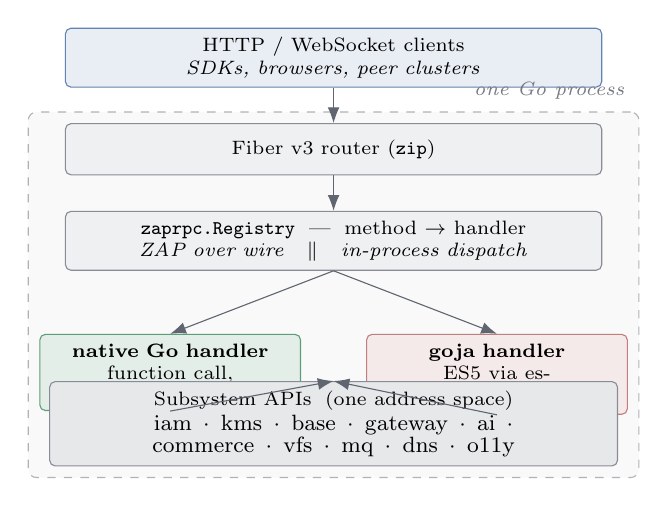
\begin{tikzpicture}[
  font=\scriptsize,
  node distance=4.5mm,
  box/.style={draw, rounded corners=2pt, align=center, minimum height=6.5mm,
              inner xsep=3pt, text width=66mm},
  layer/.style={box, fill=hzslate!8, draw=hzslate!60},
  native/.style={box, fill=hzgreen!12, draw=hzgreen!70, text width=31mm},
  js/.style={box, fill=hzred!10, draw=hzred!60, text width=31mm},
  arr/.style={-{Latex[length=2mm]}, hzslate!80, line width=0.4pt}
]

\node[layer, fill=hzblue!10, draw=hzblue!70] (clients)
  {HTTP / WebSocket clients \\ \textit{SDKs, browsers, peer clusters}};

\node[layer, below=of clients] (router)
  {Fiber~v3 router (\texttt{zip})};

\node[layer, below=of router] (registry)
  {\texttt{zaprpc.Registry} \;---\; method $\rightarrow$ handler \\
   \textit{ZAP over wire $\;\parallel\;$ in-process dispatch}};

% two handler strategies
\node[native, below left=8mm and -30mm of registry] (go)
  {\textbf{native Go handler} \\ function call, no serialization};
\node[js, below right=8mm and -30mm of registry] (js)
  {\textbf{goja handler} \\ ES5 via esbuild, interpreted};

\node[layer, below=14mm of registry, text width=70mm, fill=hzslate!12] (subsys)
  {Subsystem APIs \;(one address space)\\[1pt]
   \footnotesize iam \,$\cdot$\, kms \,$\cdot$\, base \,$\cdot$\, gateway \,$\cdot$\, ai \,$\cdot$\,
   commerce \,$\cdot$\, vfs \,$\cdot$\, mq \,$\cdot$\, dns \,$\cdot$\, o11y};

\draw[arr] (clients) -- (router);
\draw[arr] (router) -- (registry);
\draw[arr] (registry.south) -- (go.north);
\draw[arr] (registry.south) -- (js.north);
\draw[arr] (go.south) -- (subsys.north);
\draw[arr] (js.south) -- (subsys.north);

\begin{scope}[on background layer]
  \node[draw=hzslate!40, dashed, rounded corners=3pt,
        fit=(router)(registry)(go)(js)(subsys),
        inner sep=4pt, fill=hzslate!3] (binary) {};
\end{scope}
\node[hzslate!70, anchor=south east, font=\scriptsize\itshape]
  at ([xshift=-2pt,yshift=1pt]binary.north east) {one Go process};

\end{tikzpicture}
\caption{The unified binary request path. Clients reach a Fiber~v3 router;
\texttt{zaprpc.Registry} resolves each method to either a native Go handler
or a goja-evaluated handler transpiled to ES5 by esbuild. Both terminate in
the same subsystem APIs within one address space; the choice is invisible
to clients and peers.}
\label{fig:cake}
\end{figure}


\texttt{zip} is a Go module (\texttt{github.com/hanzoai/zip}) that
wraps Fiber with the seams the platform needs: a module system
(\texttt{module.go}) for mounting subsystems, lifecycle and shutdown
ordering (\texttt{closers.go}), an OpenAPI surface
(\texttt{openapi.go}) generated from the same specs that drive the
\texttt{hanzoai/openapi} registry, and---centrally---\texttt{zaprpc.Registry},
the one place where a method name resolves to a handler. The registry is
the dispatch seam shared by the in-process and over-the-wire paths.

\subsection{ZAP: one RPC, two domains}

ZAP is a capability RPC modeled on Cap'n Proto's promise
pipelining~\cite{capnproto}: a call may be issued against the
\emph{result} of an earlier, still-pending call, so a chain of dependent
operations collapses into a single round trip rather than one per step.
ZAP serves two domains from one definition.

\emph{Over the wire}, external clients speak ZAP over HTTP (request/response)
or WebSocket (bidirectional, for streaming and pipelined chains). This is
the public contract: an SDK, a browser, or a peer cluster sees a stable
method surface.

\emph{Inside the process}, the same \texttt{zaprpc.Registry} resolves a
method name directly to a Go function. A subsystem that needs identity does
not open a socket; it calls into the identity module through the registry,
and the call is an ordinary function invocation with no serialization. The
registry is the decomplecting seam: \emph{policy} (which method is exposed,
to whom) is separated from \emph{transport} (wire vs.\ in-process), and
both are separated from \emph{implementation} (Go function vs.\ goja
handler).

\subsection{esbuild as the build-time and load-time transpiler}

TypeScript and modern JavaScript do not run in \texttt{goja} directly;
\texttt{goja} targets ES5.1 with select later features. \texttt{zip}
embeds the \texttt{esbuild} Go API~\cite{esbuild} to transpile and bundle
handler sources to ES5. esbuild runs in-process (it is itself a Go
program), so transpilation needs no external toolchain and no CGO. Two
modes are supported: \emph{build-time}, where handlers are transpiled once
and embedded into the binary via \texttt{go:embed}; and \emph{load-time},
where a handler bundle is transpiled on first use and cached. Build-time is
the default for shipped code; load-time exists for development and for the
migration window (\S\ref{sec:migration}).

\subsection{No CGO, one artifact}

Both \texttt{goja} and the \texttt{esbuild} Go API are pure Go. The binary
therefore links statically with \texttt{CGO\_ENABLED=0} and cross-compiles
to every target with the standard Go toolchain---no native toolchain per
architecture, no QEMU emulation step. The same source produces an
\texttt{amd64} and an \texttt{arm64} artifact in parallel on native
runners. One artifact, parameterized by configuration, is the unit of
deployment for every brand and tenant.

\section{Migration Path}
\label{sec:migration}

The framework's purpose is to make migration \emph{incremental} and
\emph{contract-preserving}. An existing TypeScript service ports in three
stages, and the HTTP/ZAP contract is invariant across all three.

\paragraph{Stage 0 --- lift.}
The service's handlers are transpiled to ES5 with esbuild and registered in
\texttt{zaprpc.Registry} as goja-evaluated handlers. The service now runs
inside the unified binary. No handler logic changed; the wire contract is
identical. Inter-subsystem calls that previously crossed the network (e.g.\
a fetch to the identity service) are rewritten at the registry boundary to
resolve in-process, which is the only change a lift requires and is purely
additive at the seam.

\paragraph{Stage 1 --- strangle.}
Hot or contract-critical handlers are rewritten as native Go and swapped in
at the registry. Because the registry resolves a method name to whichever
implementation is bound, a Go handler and a goja handler are
interchangeable behind the same name. Rewriting proceeds one method at a
time with no flag day; at every point the binary is shippable.

\paragraph{Stage 2 --- retire.}
When the last method behind a service is native Go, the goja path and the
transpiled bundle for that service are dropped. The esbuild dependency
remains only where JavaScript handlers remain.

\paragraph{Case study: tRPC to ZAP.}
The \texttt{hanzoai/esign} service is mid-migration from
tRPC~\cite{trpc} to ZAP. tRPC's typed router maps cleanly onto the ZAP
method surface: a tRPC procedure becomes a ZAP method, and the
end-to-end type safety tRPC provides on the wire is preserved by ZAP's
schema. In the most recent round, all fourteen of fourteen routers are
served server-side through the ZAP surface (14/14), with the client
SDK retargeted from the tRPC link to the ZAP transport. The contract seen
by the frontend did not change; the transport beneath it did. This is the
strangle stage in practice: the routers were ported behind a stable
method surface without a coordinated client/server cutover.

\section{Multi-Tenancy}
\label{sec:multitenancy}

The same artifact serves \texttt{api.hanzo.ai}, \texttt{api.osage.cloud},
\texttt{api.lux.cloud}, \texttt{api.zoo.cloud}, and every white-label
tenant. Two things are configuration, not code: the \emph{brand} (logo,
title, identity issuer, default domain), resolved per request from the
hostname; and the \emph{enabled subsystem set}, resolved per deployment.
A tenant that needs identity and commerce but not inference mounts only
those modules; the binary is the same, the module graph differs.

This is the natural payoff of the module system and the registry. Mounting
a subsystem is registering its methods; not mounting it is not registering
them. Brand resolution is a middleware that reads the hostname and binds a
brand context that subsystems consult for issuer, theme, and policy. Per
HIP-0106, brand isolation is enforced at the data layer---every query is
scoped to the tenant resolved from the authenticated identity---so a single
process serving many brands never crosses tenant boundaries. The
white-label separation rules (no cross-brand logos, hostname-based brand
detection) are realized as configuration consumed by one binary, not as
forked deployments.

\section{The Code-Execution Boundary}
\label{sec:boundary}

The most important design line in this work separates \emph{in-process
evaluation of trusted code} from \emph{sandboxed execution of untrusted
code}. Conflating them is the failure mode the boundary exists to prevent.

\paragraph{In-process goja: trusted, fast, same address space.}
\texttt{goja} runs JavaScript in the binary's own address space with no
isolation boundary. That is precisely why it is appropriate only for
\emph{trusted} code: platform handlers authored by the platform team,
transpiled from the platform's own TypeScript, and shipped in the binary.
For this code, sharing the address space is the point---a goja handler
calls a Go subsystem through the registry with no serialization, and the
performance floor is a function call. goja is the right tool when the code
is trusted and the call is on the hot path (HIP-0105, the in-process
extension runtime).

\paragraph{\texttt{hanzoai/runtime}: untrusted, isolated, separate.}
User-supplied code, agent-generated code, and computer-use workloads are
\emph{untrusted} and must not share the control plane's address space. They
run in \texttt{hanzoai/runtime}, a distinct platform that isolates
execution in containers and microVMs with hardware-virtualization
boundaries in the lineage of Firecracker~\cite{firecracker} and the
isolate-per-tenant model of edge
runtimes~\cite{cloudflareworkers,wasm_serverless}. \texttt{runtime} ships
its own SDKs (Go, Python, TypeScript) and is out of scope for the control
plane binary except as a downstream callee.

\paragraph{The rule.}
Code the platform authors and trusts, on the hot path, runs in-process via
goja. Code the platform receives and cannot trust runs in \texttt{runtime}
behind a virtualization boundary. The two never swap roles. A handler is
never promoted from \texttt{runtime} into goja, and untrusted input is
never evaluated in goja. Stating the rule sharply is the contribution; the
mechanisms on each side are conventional.

\section{Cost Model}
\label{sec:cost}

We compare a representative decomposed control plane against the unified
binary. The decomposed baseline is $N$ services, each in its own container
with a sidecar proxy, joined by a service mesh; the unified case is one
container per replica. We avoid fabricated benchmarks and parameterize the
model by published overheads; the figures below are illustrative of the
\emph{shape} of the saving, not a measurement of a specific deployment.

\begin{figure*}[t]
\centering
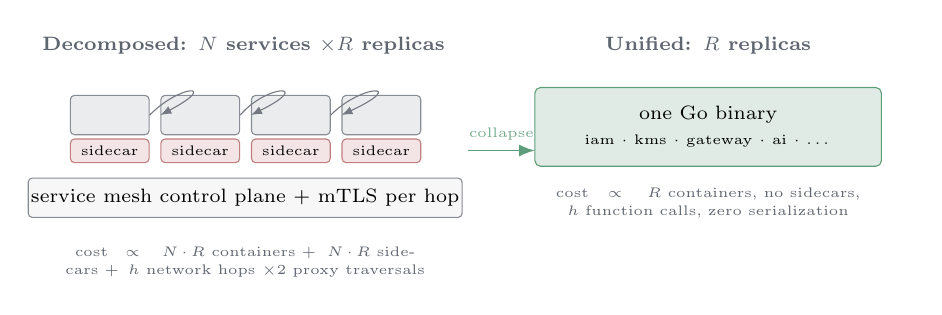
\begin{tikzpicture}[
  font=\scriptsize,
  svc/.style={draw=hzslate!60, fill=hzslate!10, rounded corners=1.5pt,
              minimum width=10mm, minimum height=5mm, inner sep=1pt},
  side/.style={draw=hzred!60, fill=hzred!12, rounded corners=1.5pt,
               minimum width=10mm, minimum height=3mm, inner sep=0pt,
               font=\fontsize{4.5}{5}\selectfont},
  one/.style={draw=hzgreen!70, fill=hzgreen!14, rounded corners=2pt,
              minimum width=44mm, minimum height=10mm, align=center},
  lbl/.style={hzslate!80}
]

% --- decomposed stack (left) ---
\node[lbl, anchor=south, font=\scriptsize\bfseries] at (1.7,2.55)
  {Decomposed: $N$ services $\times R$ replicas};

\foreach \x in {0,1,2,3} {
  \node[svc] (s\x) at (\x*1.15, 1.9) {};
  \node[side, below=0.4mm of s\x] (d\x) {sidecar};
}
\node[lbl, anchor=west, font=\fontsize{5}{6}\selectfont] at (-0.55,1.9) {};
\node[svc, fill=hzslate!4, minimum width=48mm] (mesh) at (1.72,0.85)
  {\scriptsize service mesh control plane + mTLS per hop};

\draw[-{Latex[length=1.4mm]}, hzslate!70]
  (s0.east) .. controls (0.9,2.3) and (1.4,2.3) .. (s1.west);
\draw[-{Latex[length=1.4mm]}, hzslate!70]
  (s1.east) .. controls (2.0,2.3) and (2.6,2.3) .. (s2.west);
\draw[-{Latex[length=1.4mm]}, hzslate!70]
  (s2.east) .. controls (3.2,2.3) and (3.8,2.3) .. (s3.west);

\node[lbl, anchor=north, text width=52mm, align=center,
      font=\fontsize{5.5}{6.5}\selectfont] at (1.72,0.35)
  {cost $\;\propto\; N\!\cdot\!R$ containers $+\; N\!\cdot\!R$ sidecars
   $+\; h$ network hops $\times 2$ proxy traversals};

% --- unified binary (right) ---
\node[lbl, anchor=south, font=\scriptsize\bfseries] at (7.6,2.55)
  {Unified: $R$ replicas};
\node[one] (u) at (7.6,1.75)
  {one Go binary \\[1pt]
   \fontsize{5}{6}\selectfont iam $\cdot$ kms $\cdot$ gateway $\cdot$ ai $\cdot$ \dots};
\node[lbl, anchor=north, text width=50mm, align=center,
      font=\fontsize{5.5}{6.5}\selectfont] at (7.6,1.1)
  {cost $\;\propto\; R$ containers, no sidecars, \\
   $h$ function calls, zero serialization};

\draw[-{Latex[length=2mm]}, hzgreen!70, line width=0.6pt]
  (4.55,1.45) -- node[above, font=\fontsize{5.5}{6}\selectfont, hzgreen!60]{collapse} (5.4,1.45);

\end{tikzpicture}
\caption{Illustrative cost comparison (shape, not measurement). The
decomposed stack pays for $N\!\cdot\!R$ containers plus an equal number of
sidecars and a mesh control plane; each user action crossing $h$ subsystems
pays $h$ network hops with two proxy traversals each. The unified binary
pays for $R$ containers and turns the $h$ hops into $h$ function calls.
Per-hop mesh overheads are taken from published service-mesh
measurements~\cite{istio_overhead}; the comparison assumes co-scaled
subsystems (\S\ref{sec:cost}).}
\label{fig:cost}
\end{figure*}


\paragraph{Container and proxy footprint.}
The decomposed stack pays, per service, for a container runtime slice and a
sidecar. With $N$ services and $R$ replicas, that is $N\cdot R$ application
containers \emph{plus} $N\cdot R$ sidecars; the unified binary pays for
$R$ containers and no sidecars. The sidecar CPU and memory reservation is
a fixed tax per pod that the service-mesh literature measures in the
hundreds of millicores and tens to low-hundreds of megabytes under
load~\cite{istio_overhead}; multiplied by $N\cdot R$ it is the dominant
avoidable cost.

\paragraph{Per-call overhead.}
Let a user action touch $h$ subsystems on its critical path. The decomposed
stack pays $h$ network hops, each with two proxy traversals and a
serialize/deserialize pair; the unified binary pays $h$ function calls and
zero serializations. With per-hop mesh overhead measured in the low
single-digit milliseconds~\cite{istio_overhead}, a four-subsystem action
sheds several milliseconds of pure overhead and the CPU that produced it.

\paragraph{Operational surface.}
$N$ pipelines, $N$ rollouts, $N$ dashboards, and a mesh control plane
collapse to one pipeline, one rollout, and one process to observe. This is
not a compute cost but it is a real and recurring engineering cost; the
DeathStarBench and service-mesh studies both note operational complexity as
a first-order property of microservice topologies~\cite{deathstarbench,istio_overhead}.

\paragraph{What the unified binary does \emph{not} save.}
It does not reduce the work the application actually performs, and it does
not help when subsystems must scale independently---if inference needs ten
times the replicas of identity, co-locating them wastes the smaller
subsystem's headroom. The model assumes co-scaling, which holds for the
control plane and fails for the inference data plane; the latter is
deployed separately for exactly this reason.

\section{Performance}
\label{sec:perf}

\paragraph{Function call vs.\ network RPC.}
The structural performance argument is that an in-process subsystem call is
a Go function invocation---nanoseconds, no allocation beyond arguments, no
serialization---against a network RPC's microseconds-to-milliseconds of
serialize, syscall, network, deserialize, and (with a mesh) two proxy
traversals. The unified binary moves every co-located call from the latter
class to the former. The latency floor of an intra-binary call is set by
Go's call and scheduling cost, not by the network stack.

\paragraph{Promise pipelining at the edge.}
For calls that \emph{do} cross the network---external clients, peer
clusters---ZAP's promise pipelining~\cite{capnproto} collapses dependent
call chains into a single round trip. A client that creates a resource and
immediately operates on it issues the second call against the promise of
the first; the server resolves the chain locally. This bounds edge latency
by one round trip per dependent chain rather than one per call, which is
the same economy the in-process path gets for free, recovered for the cases
that must remain remote.

\paragraph{goja overhead, honestly.}
A goja-evaluated handler is slower than the equivalent native Go handler:
it interprets ECMAScript and bridges values across the Go/JS boundary. This
is the cost of Stage~0 (\S\ref{sec:migration}) and the reason Stage~1
exists. The design does not pretend goja is free; it makes the goja path a
\emph{temporary} state that the strangle stage retires on the hot path
while keeping the cold path in JavaScript as long as that is cheaper to
maintain than to rewrite.

\section{Future Work}
\label{sec:future}

Three directions extend the framework without changing its shape. First,
\emph{additional in-process language runtimes}---a \texttt{pyvm} and a
\texttt{v8vm} mounted behind the same registry seam---so trusted handlers
in Python or via a V8 isolate dispatch identically to goja handlers, with
the isolate option offering a stronger in-process boundary than goja for
code that is trusted but warrants defense in depth. Second,
\emph{hot reload} of goja modules: because load-time transpilation already
exists, swapping a handler bundle without restarting the process is a
registry rebinding, useful in development and for cold-path handlers.
Third, \emph{gRPC-on-ZAP interop}~\cite{grpc}, exposing the ZAP surface to
gRPC clients so existing gRPC ecosystems consume the platform without a new
SDK, and \emph{deeper observability}, attributing power and CPU to
in-process subsystems with the granularity that tools such as
Kepler~\cite{kepler} bring to containers---harder inside one process,
and the right place to invest the operational savings the unified binary
returns.

\section{Conclusion}

For a co-located, co-released control plane, decomposition into networked
microservices spends compute on proxies and serialization, adds latency in
proportion to the hop count, and imposes a distributed-systems tax with no
scaling benefit to justify it. The Hanzo unified cloud binary collapses the
control plane into one Go process: \texttt{zip} over Fiber~v3, ZAP serving
both the wire and the in-process dispatch seam, goja and esbuild admitting
TypeScript backends without a rewrite, and a strangle path to native Go
that never breaks the contract. One artifact serves every brand and tenant
by configuration. The boundary against untrusted code---in-process goja for
trusted hot paths, the sandboxed \texttt{runtime} for everything else---is
the load-bearing design decision, and we have stated it sharply. The saving
is not magic; it is the removal of plumbing that the workload never needed.

{\small
\bibliographystyle{plain}
\bibliography{references}
}

\end{document}
